\documentclass[a4paper,12pt,oneside]{book}

%-------------------------------Start of the Preable------------------------------------------------
\usepackage[english]{babel}
\usepackage{blindtext}
%packagr for hyperlinks
\usepackage{hyperref}
\hypersetup{
    colorlinks=true,
    linkcolor=blue,
    filecolor=magenta,      
    urlcolor=cyan,
}

\urlstyle{same}
%use of package fancy header
\usepackage{fancyhdr}
\setlength\headheight{26pt}
\fancyhf{}
%\rhead{
\includegraphics[width=1cm]{logo}}
\lhead{\rightmark}
\rhead{
\includegraphics[width=1cm]{logo}}
\fancyfoot[RE, RO]{\thepage}
\fancyfoot[CE, CO]{\href{http://www.e-yantra.org}{www.e-yantra.org}}

\pagestyle{fancy}

%use of package for section title formatting
\usepackage{titlesec}
\titleformat{\chapter}
  {\Large\bfseries} % format
  {}                % label
  {0pt}             % sep
  {\huge}           % before-code
 
%use of package tcolorbox for colorful textbox
\usepackage[most]{tcolorbox}
\tcbset{colback=cyan!5!white,colframe=cyan!75!black,halign title = flush center}

\newtcolorbox{mybox}[1]{colback=cyan!5!white,
colframe=cyan!75!black,fonttitle=\bfseries,
title=\textbf{\Large{#1}}}

%use of package marginnote for notes in margin
\usepackage{marginnote}

%use of packgage watermark for pages
%\usepackage{draftwatermark}
%\SetWatermarkText{
\includegraphics{logo}}
\usepackage[scale=2,opacity=0.1,angle=0]{background}
\backgroundsetup{
contents={
\includegraphics{logo}}
}

%use of newcommand for keywords color
\usepackage{xcolor}
\newcommand{\keyword}[1]{\textcolor{red}{\textbf{#1}}}

%package for inserting pictures
\usepackage{graphicx}
\graphicspath{{./images/}}
%package for highlighting
%\usepackage{color,soul}

%new command for table
\newcommand{\head}[1]{\textnormal{\textbf{#1}}}


%----------------------End of the Preamble---------------------------------------


\begin{document}

%---------------------Title Page------------------------------------------------
\begin{titlepage}
\raggedright
{\Large eYSIP2017\\[1cm]}
{\Huge\scshape Indoor Environment Mapping Using UAV \\[.1in]}
\vfill
\begin{flushright}
{\large Rishabh Beri \\}
{\large Samaahita S Belavadi \\}
{\large Mentors: Simranjeet, Vamshi \\}
{\large Duration of Internship: $ 22/05/2017-07/07/2017 $ \\}
\end{flushright}

{\itshape 2017, e-Yantra Publication}
\end{titlepage}
%-------------------------------------------------------------------------------

\chapter[Project Tag]{Indoor Environment Mapping Using UAV}
\section*{Abstract}
Research in the area of robotic indoor mapping has been active for a very long time. This project aims to solve the problem of autonomous mapping of an indoor environment using an unmanned aerial vehicle. The platform chosen to solve this problem is Robotics Operating System(ROS) and Gazebo simulator. \\
ROS is an open-source system for controlling robots via PC. It has various libraries and packages that simplify the task of building robotic software applications. \\
Gazebo is a simulator powered with a physics engine, used to simulate the real world. It enables setting of parameters like gravity, friction, inertia, etc. to replicate any real world scenario. \\
The package used for map building is RTAB-Map which runs an RGB-D Graph SLAM algorithm based on the global Bayesian loop closure detector. \\
In simulation, this problem was solved using an Intel Realsense R200 camera mounted on an AR Drone 2.0. In the real world, we used a Kinect v1.0 camera mounted on a Firebird VI robot, which is controlled manually.

\subsection*{Completion status}
\begin{itemize}
	\item Completed autonomous mapping in simulation
	\item Interfaced Kinect camera with the PC
	\item Completed manual mapping in the real world
	\item Made tutorials on the various packages used in the project
	\item Video explaining the autonomous mapping algorithm used
\end{itemize}

\section{Hardware Components}
\begin{itemize}  
  \item Kinect v1.0 (\href{https://en.wikipedia.org/wiki/Kinect#Kinect_for_Xbox_360_.28V1_2010.29}{Specifications})
  
  \item Firebird VI (\href{https://github.com/eYSIP-2017/eYSIP-2017_Indoor-Environments-Mapping-using-UAV/tree/master/Documents/Firebird-VI}{Datasheets and Manuals}, \href{http://www.nex-robotics.com/products/fire-bird-vi-robot/fire-bird-vi-robotic-research-platform.html}{Buy here})
  
  \item USB to RS-232 Converter (\href{{./datasheet/USB to RS-232 Converter.pdf}}{Datasheet}, \href{http://www.nex-robotics.com/products/usb-interfacing/usb-to-rs-232-converter.html}{Buy here})  	
\end{itemize}

\begin{figure}[h]
	\centering
	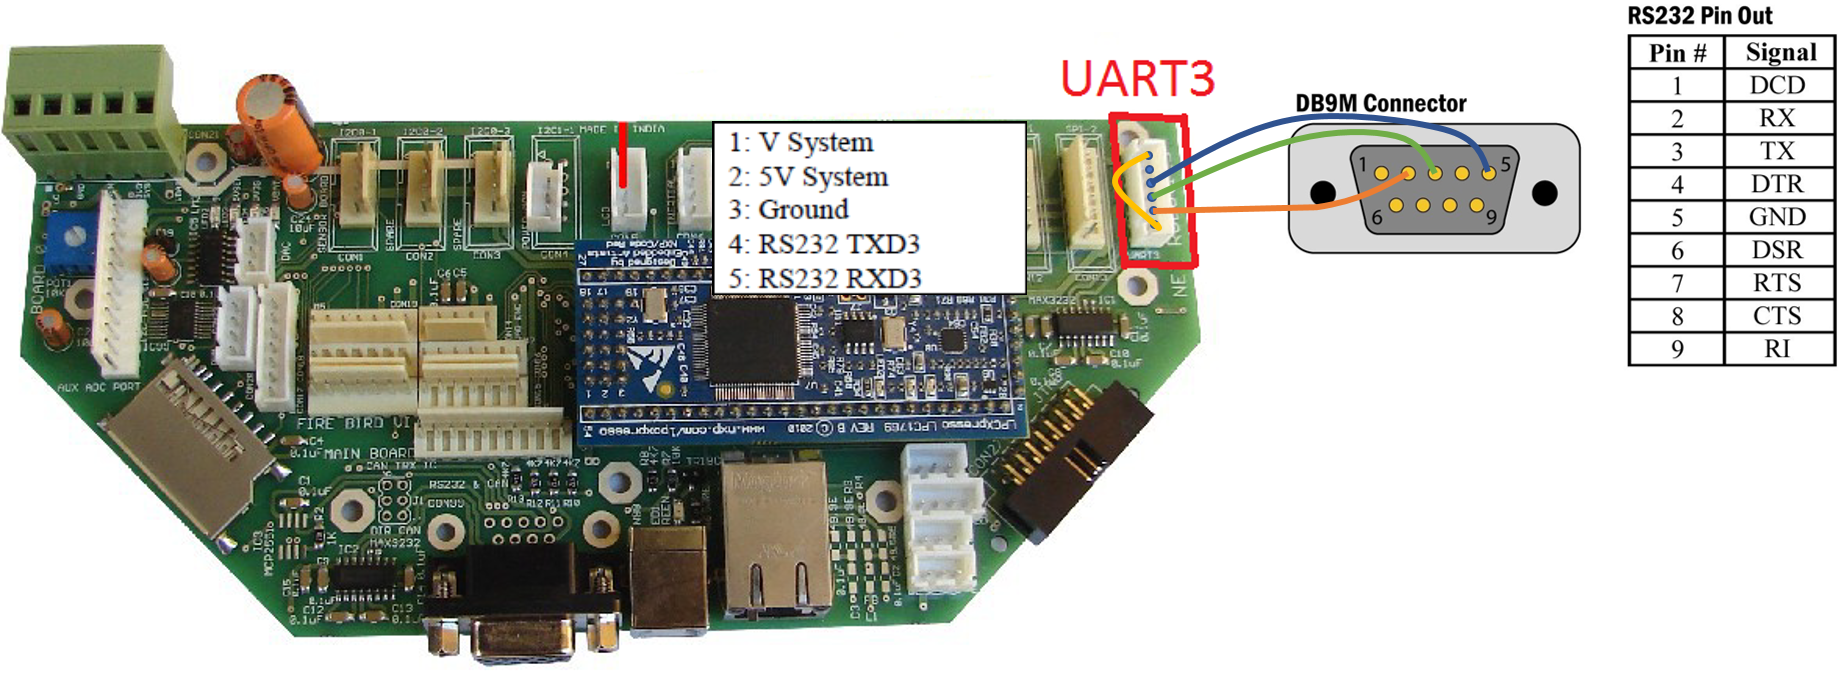
\includegraphics[scale=0.25]{circuit}
	\caption{Circuit Diagram}
\end{figure}

\section{Software used}
\begin{itemize}  
  \item Ubuntu
  \begin{itemize}
  	\item Version - 14.04
  \end{itemize}
  
  \item ROS
  \begin{itemize}
  	\item Version - Indigo
  	\item Installation: \\
  	\texttt{sudo apt-get install ros-indigo-desktop-full}
  \end{itemize}   
  
  \item Gazebo Simulator
  \begin{itemize}
  	\item Version - 7
  	\item Installation - Download and run \href{https://github.com/eYSIP-2017/eYSIP-2017_Indoor-Environments-Mapping-using-UAV/blob/master/bash_scripts/install_gazebo7.sh}{this} file to install gazebo7
  \end{itemize}
  
\end{itemize}

\section{The Mapping Process}

\begin{figure}[h]
	\centering
	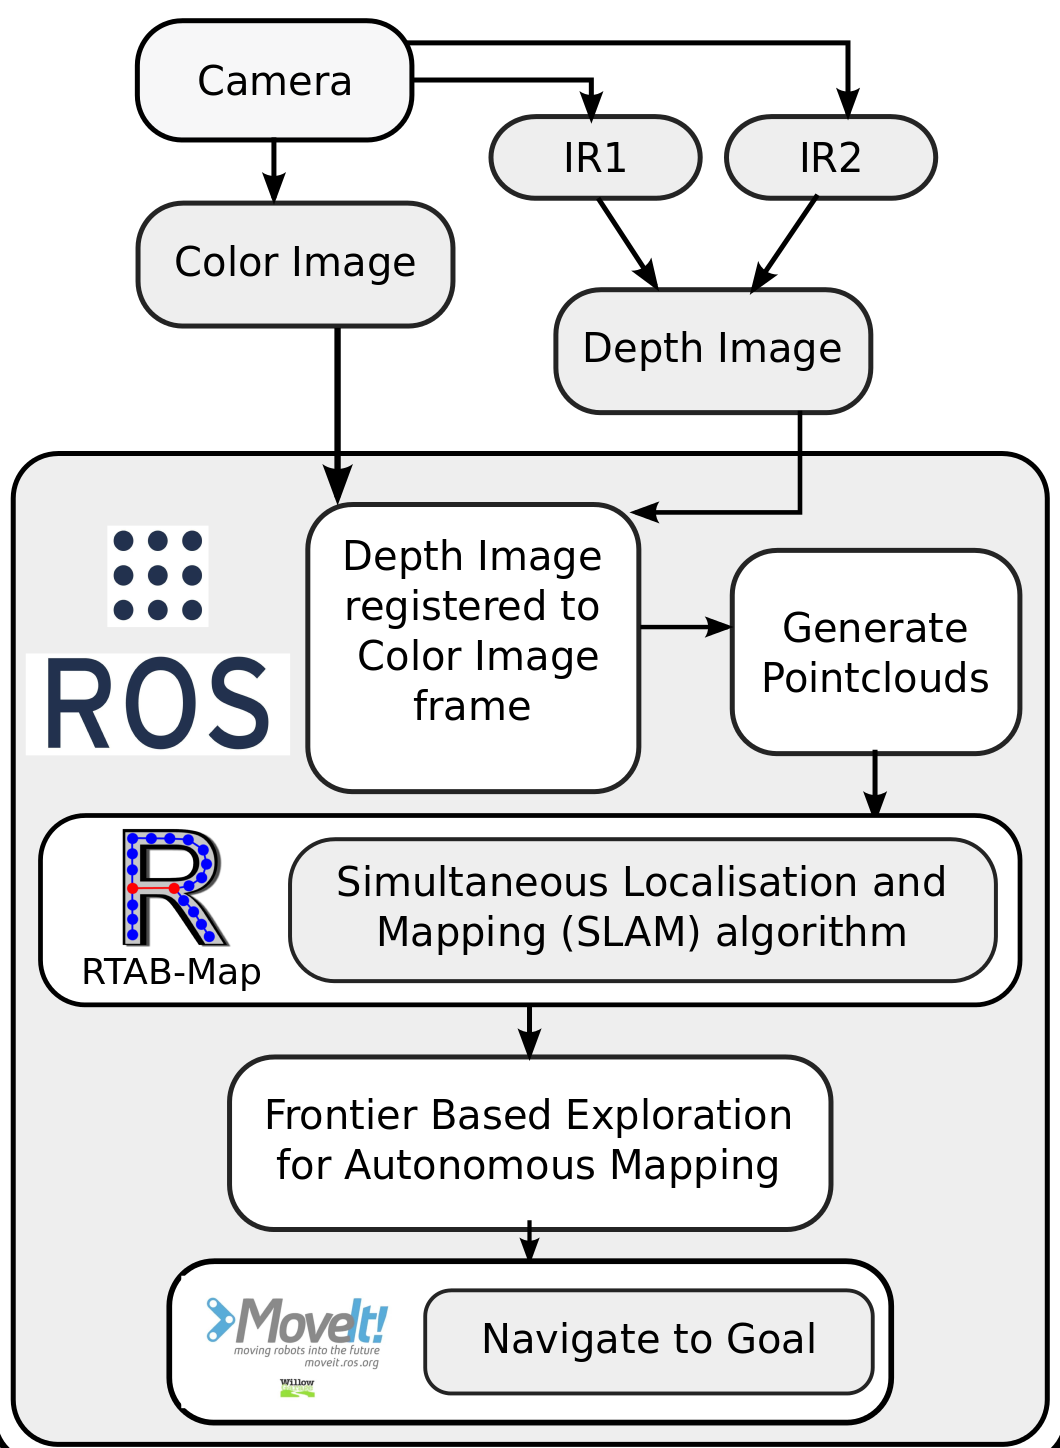
\includegraphics[scale=0.27]{process}
	\caption{The mapping process}
\end{figure}

\subsection*{Packages Required}
\begin{itemize}
	\item ardrone\_simulator\_gazebo7 - This package contains the models, drivers and plug-ins necessary to simulate the behaviour of an AR Drone in Gazebo7. 

	\item depth\_image\_proc - This package is a part of the image pipeline package of ROS, and contains nodelets for processing depth images.
		
	\item realsense\_gazebo\_plugin	- This package contains the models, drivers and plugins necessary to simulate the behaviour of an Intel Realsense R200 camera in Gazebo7.
		
	\item move\_it - This package plans the path of the drone from it's current location to a goal point.		
		
\end{itemize}

\subsection*{Initial Setup}
\begin{itemize}
	\item Including the drone and camera in gazebo
		\begin{itemize}
			\item The model of the AR Drone is in the URDF format
			\item But, the model of the Realsense camera is in SDF format
			\item URDF and SDF formats are incompatible. Hence, one format has to be converted to the other
			\item \href{https://github.com/eYSIP-2017/eYSIP-2017_Indoor-Environments-Mapping-using-UAV/blob/master/Documents/Tutorials/Adding%20Realsense%20R200%20camera%20to%20ARDrone%20in%20Gazebo7.pdf}{This} tutorial explains the conversion process
		\end{itemize}
\end{itemize}

\vspace{.5in}

\begin{figure}[h]
	\centering
	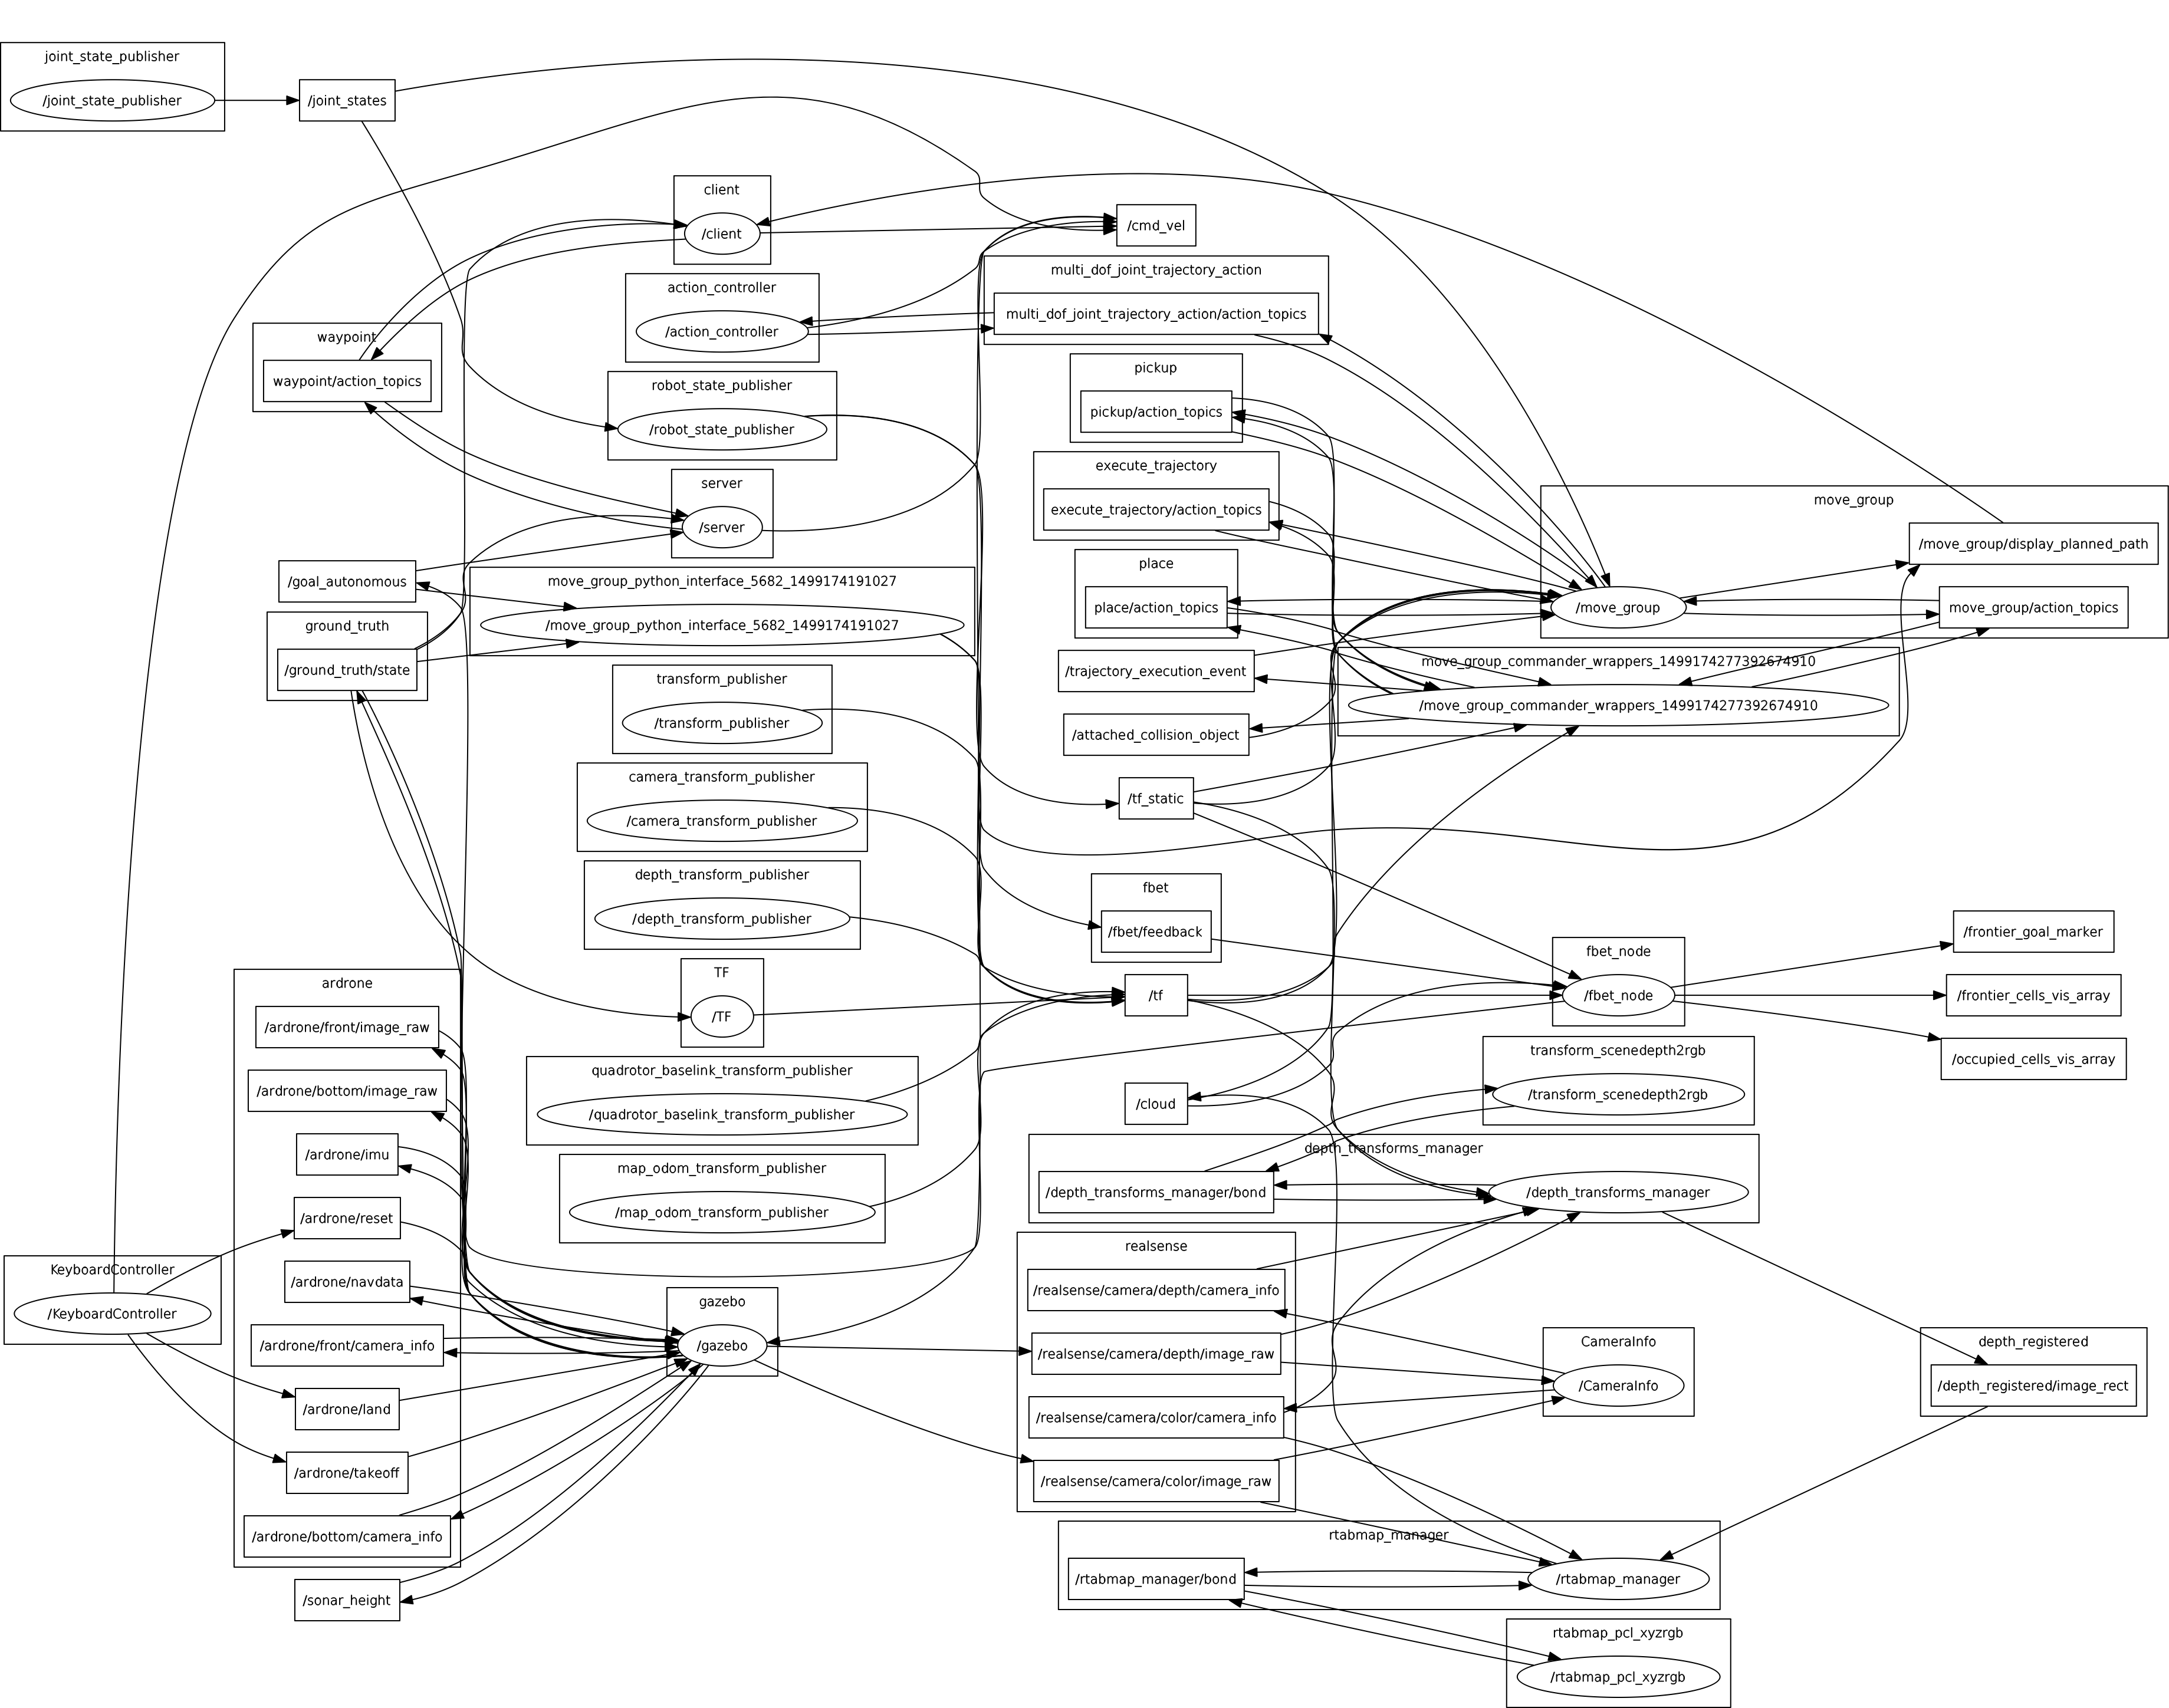
\includegraphics[scale=0.14]{rosgraph}
	\caption{Output of the rqt\_graph command showing how the nodes communicate with each other}
\end{figure}
	
\subsection*{Generation of Pointclouds}
\begin{itemize}

	\item Register (i.e. project) the depth image to the frame of the colour image
		\begin{itemize}
			\item The realsense camera publishes RGB and depth images on topics /realsense/camera/color/image\_raw and /realsense/camera/depth/image\_raw respectively
			\item But to generate an RGB-D pointcloud, the depth image and the colour image have to be in the same frame.
			\item The register nodelet (i.e., depth\_registered in rqt\_graph) of the depth\_image\_proc package is used for registering the depth image to the frame of the colour image
			\item Requirements:
				\begin{itemize}
					\item Meta-data of the RGB camera (Published on the topic /realsense/camera/color/camera\_info)
					\item Meta-data of the depth camera (Published on the topic /realsense/camera/depth/camera\_info)
					\item Depth Image (Published on the topic /realsense/camera/depth/image\_raw)
					\item A transform between the frame of the depth camera and that of the colour camera (A static transform between color and depth published on the topic /tf)
				\end{itemize}
			\item The output of this nodelet is a registered depth image (Published on the topic /depth\_registered/image\_rect)
		\end{itemize}
	
	\item Create a pointcloud
		\begin{itemize}
			\item The point\_cloud\_xyzrgb nodelet (i.e., rtabmap\_pcl\_xyzrgb in the rqt\_graph) of the rtabmap\_ros package is used to generate a pointcloud in which each point has 7 attributes - 3D co-ordinates, RGB-colour and depth.
			\item Requirements:
				\begin{itemize}
					\item RGB image (Published on the topic /realsense/camera/color/image\_raw)
					\item Registered depth image (Published on the topic /depth\_registered/image\_rect)
					\item Meta-data of the RGB camera (Published on the topic /realsense/camera/color/camera\_info)
				\end{itemize}
			\item The output of this nodelet is a pointcloud (Published on the topic /cloud)
		\end{itemize}
		
\end{itemize}

\begin{figure}[h]
	\centering
	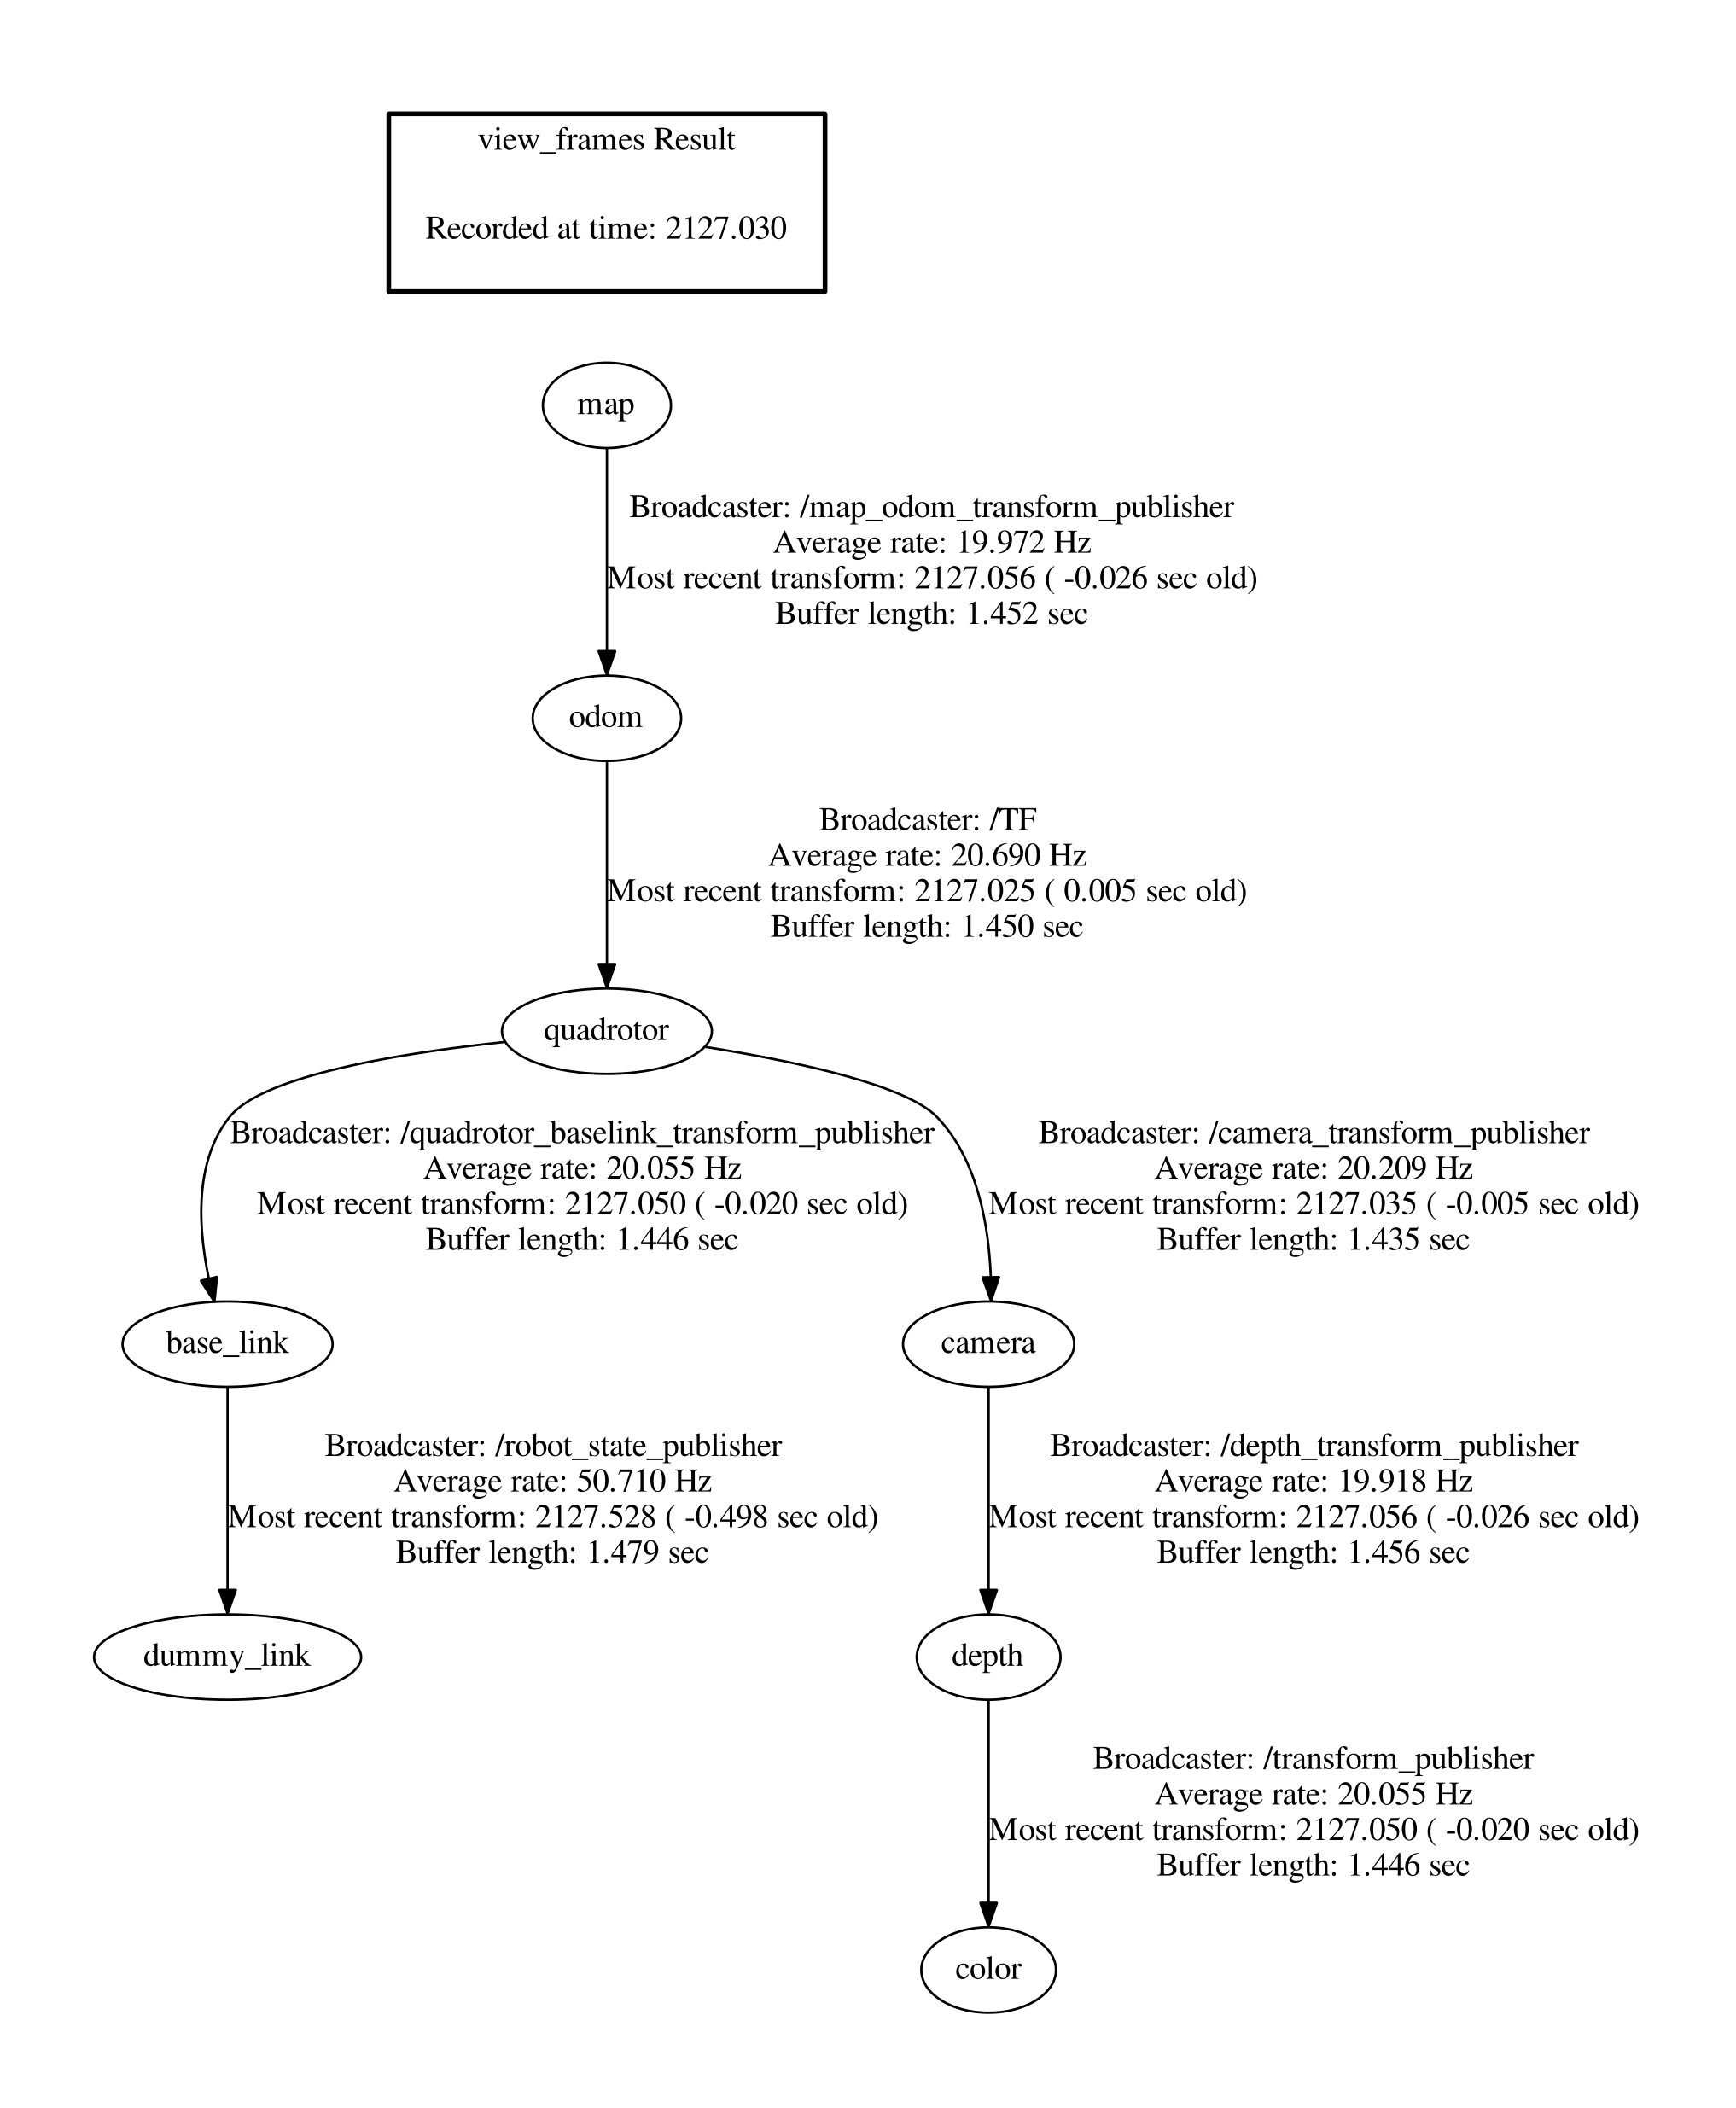
\includegraphics[scale=0.15]{tftree}
	\caption{The tf tree generated during the mapping process}
\end{figure}

\subsection*{Map Building using RTAB-Map}
\begin{itemize}

	\item SLAM - Simultaneous Localization and Mapping \\
	Simultaneous Localization and Mapping (SLAM), is the problem of building the map of an unknown environment incrementally, while simultaneously keeping track of a robot's location within the map. \\
	The SLAM algorithm applied depends on the sensors used in the mapping process. These algorithms are broadly classified into landmark-based and raw-data algorithms. Landmark-based algorithms uniquely identify objects in the world, whose location is estimated using a sensor. Raw-data algorithms on the other hand, model the probability of estimating the correctness of an observation directly as a function of the location. \\
	RTAB-Map is a RGB-D Graph SLAM approach based on the global Bayesian loop closure detector. Loop-Closure is the problem of identifying a previously visited location based on sensed features and updating the variables accordingly. The loop closure detector uses a bag-of-words approach to determinate how likely a new image comes from a previous location or a new location.	

	\item The main node of the RTAB-Map package is rtabmap
	\item The map is incrementally built and optimized whenever a loop-closure is detected
	\item Requirements:
		\begin{itemize}
			\item Odometry information (Published on the topic /ground\_truth/state)
			\item RGB image (Published on the topic /realsense/camera/color/image\_raw)
			\item Metadata of the RGB image (Published on the topic /realsense/camera/color/camera\_info)
			\item Registered depth image (Published on the topic /depth\_registered/image\_rect)
			\item Pointclouds (Published on the topic /cloud)
		\end{itemize}
	\item The output of this node is an incrementally built map and information about the map
	\item There are various parameters that can be set to use the node for a wide variety of applications (More information about these parameters can be found \href{http://wiki.ros.org/rtabmap_ros#rtabmap}{here})
	\item \href{https://github.com/eYSIP-2017/eYSIP-2017_Indoor-Environments-Mapping-using-UAV/blob/master/Documents/Tutorials/Using%20RTAB-Map%20for%20mapping%20with%20Kinect.pdf}{This} tutorial explains how to use RTAB-Map for mapping

\end{itemize}

\subsection*{Autonomous Mapping - Frontier-Based Exploration Technique (FBET)}
\begin{itemize}
	\item Algorithm for Goal generation:
	\begin{enumerate}
		\item Receive a Pointcloud (Published on the topic /cloud)
		\item Convert the Pointcloud to an Octomap 
		\item Classify cells in the Octomap as free or occupied
		\item Find frontier cells
		\begin{itemize}
			\item Frontier cells represent the boundary of known and unknown regions
			\item A free cell is a frontier cell if it has one free cell and one unknown cell as it's neighbour
		\end{itemize}
		\item Cluster the frontier cells using the k-means clustering algorithm
			\begin{itemize}
				\item The number of clusters 'k', depends upon the number of frontier cells
				\item Since the camera has a limited field of view, we limit the number of frontier cells each cluster can accommodate
			\end{itemize}
		\item Calculate the cost of each cluster. The cost function depends on:
		\begin{itemize}
			\item Inverse of the cluster size - Cluster size represents the size of the unknown region
			\item Distance between the drone and the centroid of the cluster
		\end{itemize}
		\item The cluster with the minimum cost is chosen the optimal cluster
		\item The centroid of the optimal cluster is the new goal to navigate to (This new goal is published on the topic /goal\_autonomous)
	\end{enumerate}
	
	\item Path planning
		\begin{itemize}
			\item Package used - MoveIt
			\item MoveIt is a ROS framework used for motion planning, control and navigation of robotic arms
			\item By making a few changes, we can use it for planning the path of a quadrotor too
			\item If it is not possible for MoveIt to generate a path to a goal(Goal is too close to an obstacle), then a feedback mechanism requests the autonomous\_exploration node for a new goal (The feedback is sent by sending an empty message to the autonomous\_exploration node over the topic /fbet/feedback whenever MoveIt is unable to generate a plan)
		\end{itemize}

	\item Navigating to the goal
		\begin{itemize}
			\item Once a plan has been generated, we use actionlib server-client mechanism along with PID control to navigate through each waypoint of the goal (These waypoints are extracted from the topic /move\_group/display\_planned\_path)
		\end{itemize}
		
	\item \href{https://youtu.be/Ow4pZlDPhkY}{This} video explains the mapping process			
	
\end{itemize}

\pagebreak

\section{Software and Code}
\href{https://github.com/eYSIP-2017/eYSIP-2017_Indoor-Environments-Mapping-using-UAV}{Github link} for the repository of code

\begin{itemize}

	\item /ardrone\_simulator\_gazebo7/cvg\_sim\_gazebo/scripts/aruco\_land.py - Script to execute landing of the drone on an ArUco marker.

	\item /ardrone\_simulator\_gazebo7/cvg\_sim\_gazebo/scripts/keyboard.py - Script to control the drone manually
	
	\item /ardrone\_simulator\_gazebo7/cvg\_sim\_gazebo/scripts/ardrone\_get\_odometry.py - Script to fetch pose of the drone from gazebo and publish tf
	
	\item /realsense\_gazebo\_plugin/scripts/pub\_camera\_info.py - Publish fake depth and color camera info for the simulated cameras
	
	\item /realsense\_gazebo\_plugin/scripts/server.py - Start the actionlib server to execute the waypoints from MoveIt!
	
	\item /realsense\_gazebo\_plugin/scripts/client.py - Start the actionlib client to execute the waypoints from MoveIt!
	
	\item /realsense\_gazebo\_plugin/scripts/send\_goal.py - Start the script to send goals to MoveIt!
	
	\item /realsense\_gazebo\_plugin/launch/ardrone\_realsense.launch - Launch Gazebo7 and load the simulated world
	
	\item /realsense\_gazebo\_plugin/launch/register.launch - Register the depth image to the color image frame
	
	\item /realsense\_gazebo\_plugin/launch/rtabmap\_pcl.launch - Launch nodelet to convert depth and color image to pointcloud
	
	\item /realsense\_gazebo\_plugin/launch/fbet.launch - Launch the autonomous\_exploration node which runs the FBET algorithm
	
	\item /move\_it/launch/moveit.launch - Launch the MoveIt! path planner
	
	\item /autonomous\_exploration/src/autonomous\_exploration.cpp - Code to find goals for autonomous navigation	
	
	\item /bash\_scripts/keyboard\_mapping.sh - Bash script to launch all necessary packages required for the mapping process
	
\end{itemize}

\section{Tutorials}
\begin{itemize}
	\item \href{https://github.com/eYSIP-2017/eYSIP-2017_Indoor-Environments-Mapping-using-UAV/blob/master/Documents/Tutorials/Adding%20Realsense%20R200%20camera%20to%20ARDrone%20in%20Gazebo7.pdf}{Adding Realsense R200 camera to ARDrone in Gazebo7}
	\item \href{https://github.com/eYSIP-2017/eYSIP-2017_Indoor-Environments-Mapping-using-UAV/blob/master/Documents/Tutorials/Landing%20Drone%20on%20ArUco%20marker.pdf}{Landing Drone on ArUco marker}
	
	\item \href{https://github.com/eYSIP-2017/eYSIP-2017_Indoor-Environments-Mapping-using-UAV/blob/master/Documents/Tutorials/OctoMap%20and%20RTAB-Map.pdf}{OctoMap and RTAB-Map}
	
	\item \href{https://github.com/eYSIP-2017/eYSIP-2017_Indoor-Environments-Mapping-using-UAV/blob/master/Documents/Tutorials/Using%20RTAB-Map%20for%20mapping%20with%20Kinect.pdf}{Using RTAB-Map for mapping with Kinect}
	
	\item \href{https://github.com/eYSIP-2017/eYSIP-2017_Indoor-Environments-Mapping-using-UAV/blob/master/Documents/Tutorials/Keyboard%20Mapping.pdf}{Keyboard Mapping}
	
	\item \href{https://github.com/eYSIP-2017/eYSIP-2017_Indoor-Environments-Mapping-using-UAV/blob/master/Documents/Tutorials/Autonomous%20Mapping.pdf}{Autonomous Mapping}
	
\end{itemize}

\vspace{.5in}

\section{Results and Demo}
\begin{figure}[h]
	\centering
	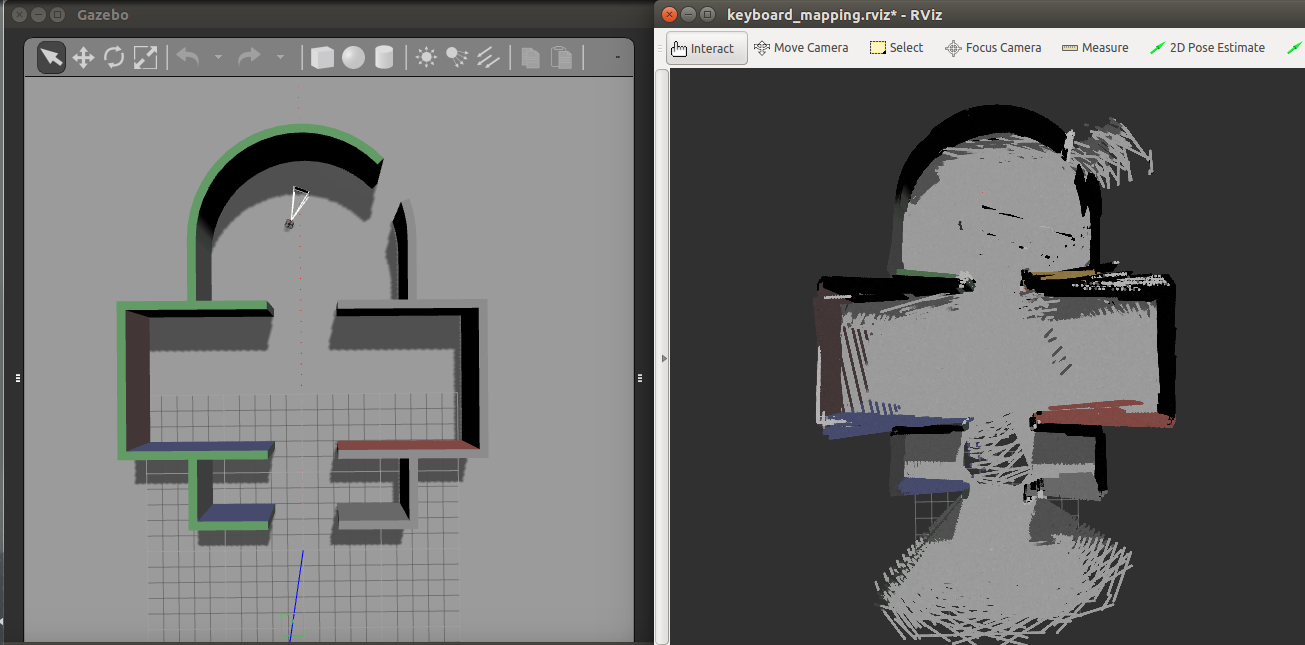
\includegraphics[scale=0.28]{map}
	\caption{Result of manual mapping in simulation}
\end{figure}

\href{https://youtu.be/cg0Gf3kulE8}{Demonstration video for manual mapping in simulation}

\pagebreak

\begin{figure}[h]
	\centering
	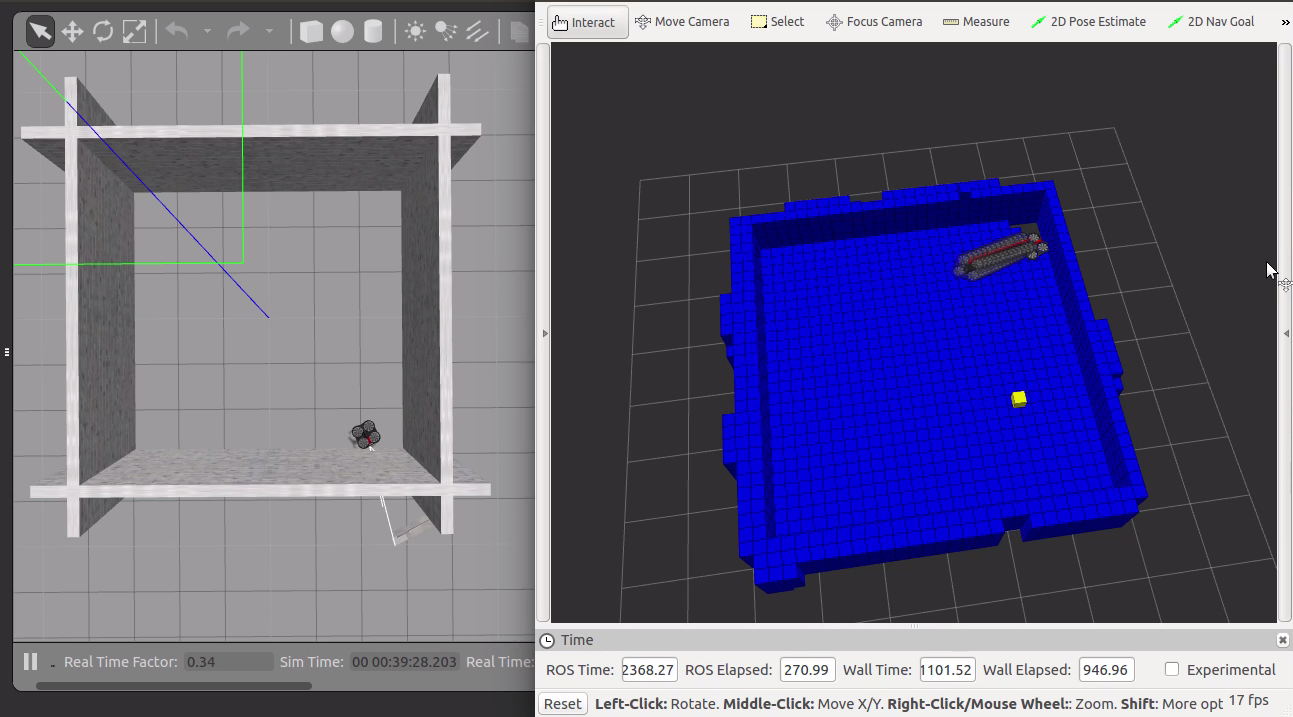
\includegraphics[scale=0.35]{automap}
	\caption{Result of autonomous mapping in simulation}
\end{figure}

\href{https://youtu.be/kXyV3OpbWo8}{Demonstration video for autonomous mapping in simulation}

\vspace{1in}

\begin{figure}[h]
	\centering
	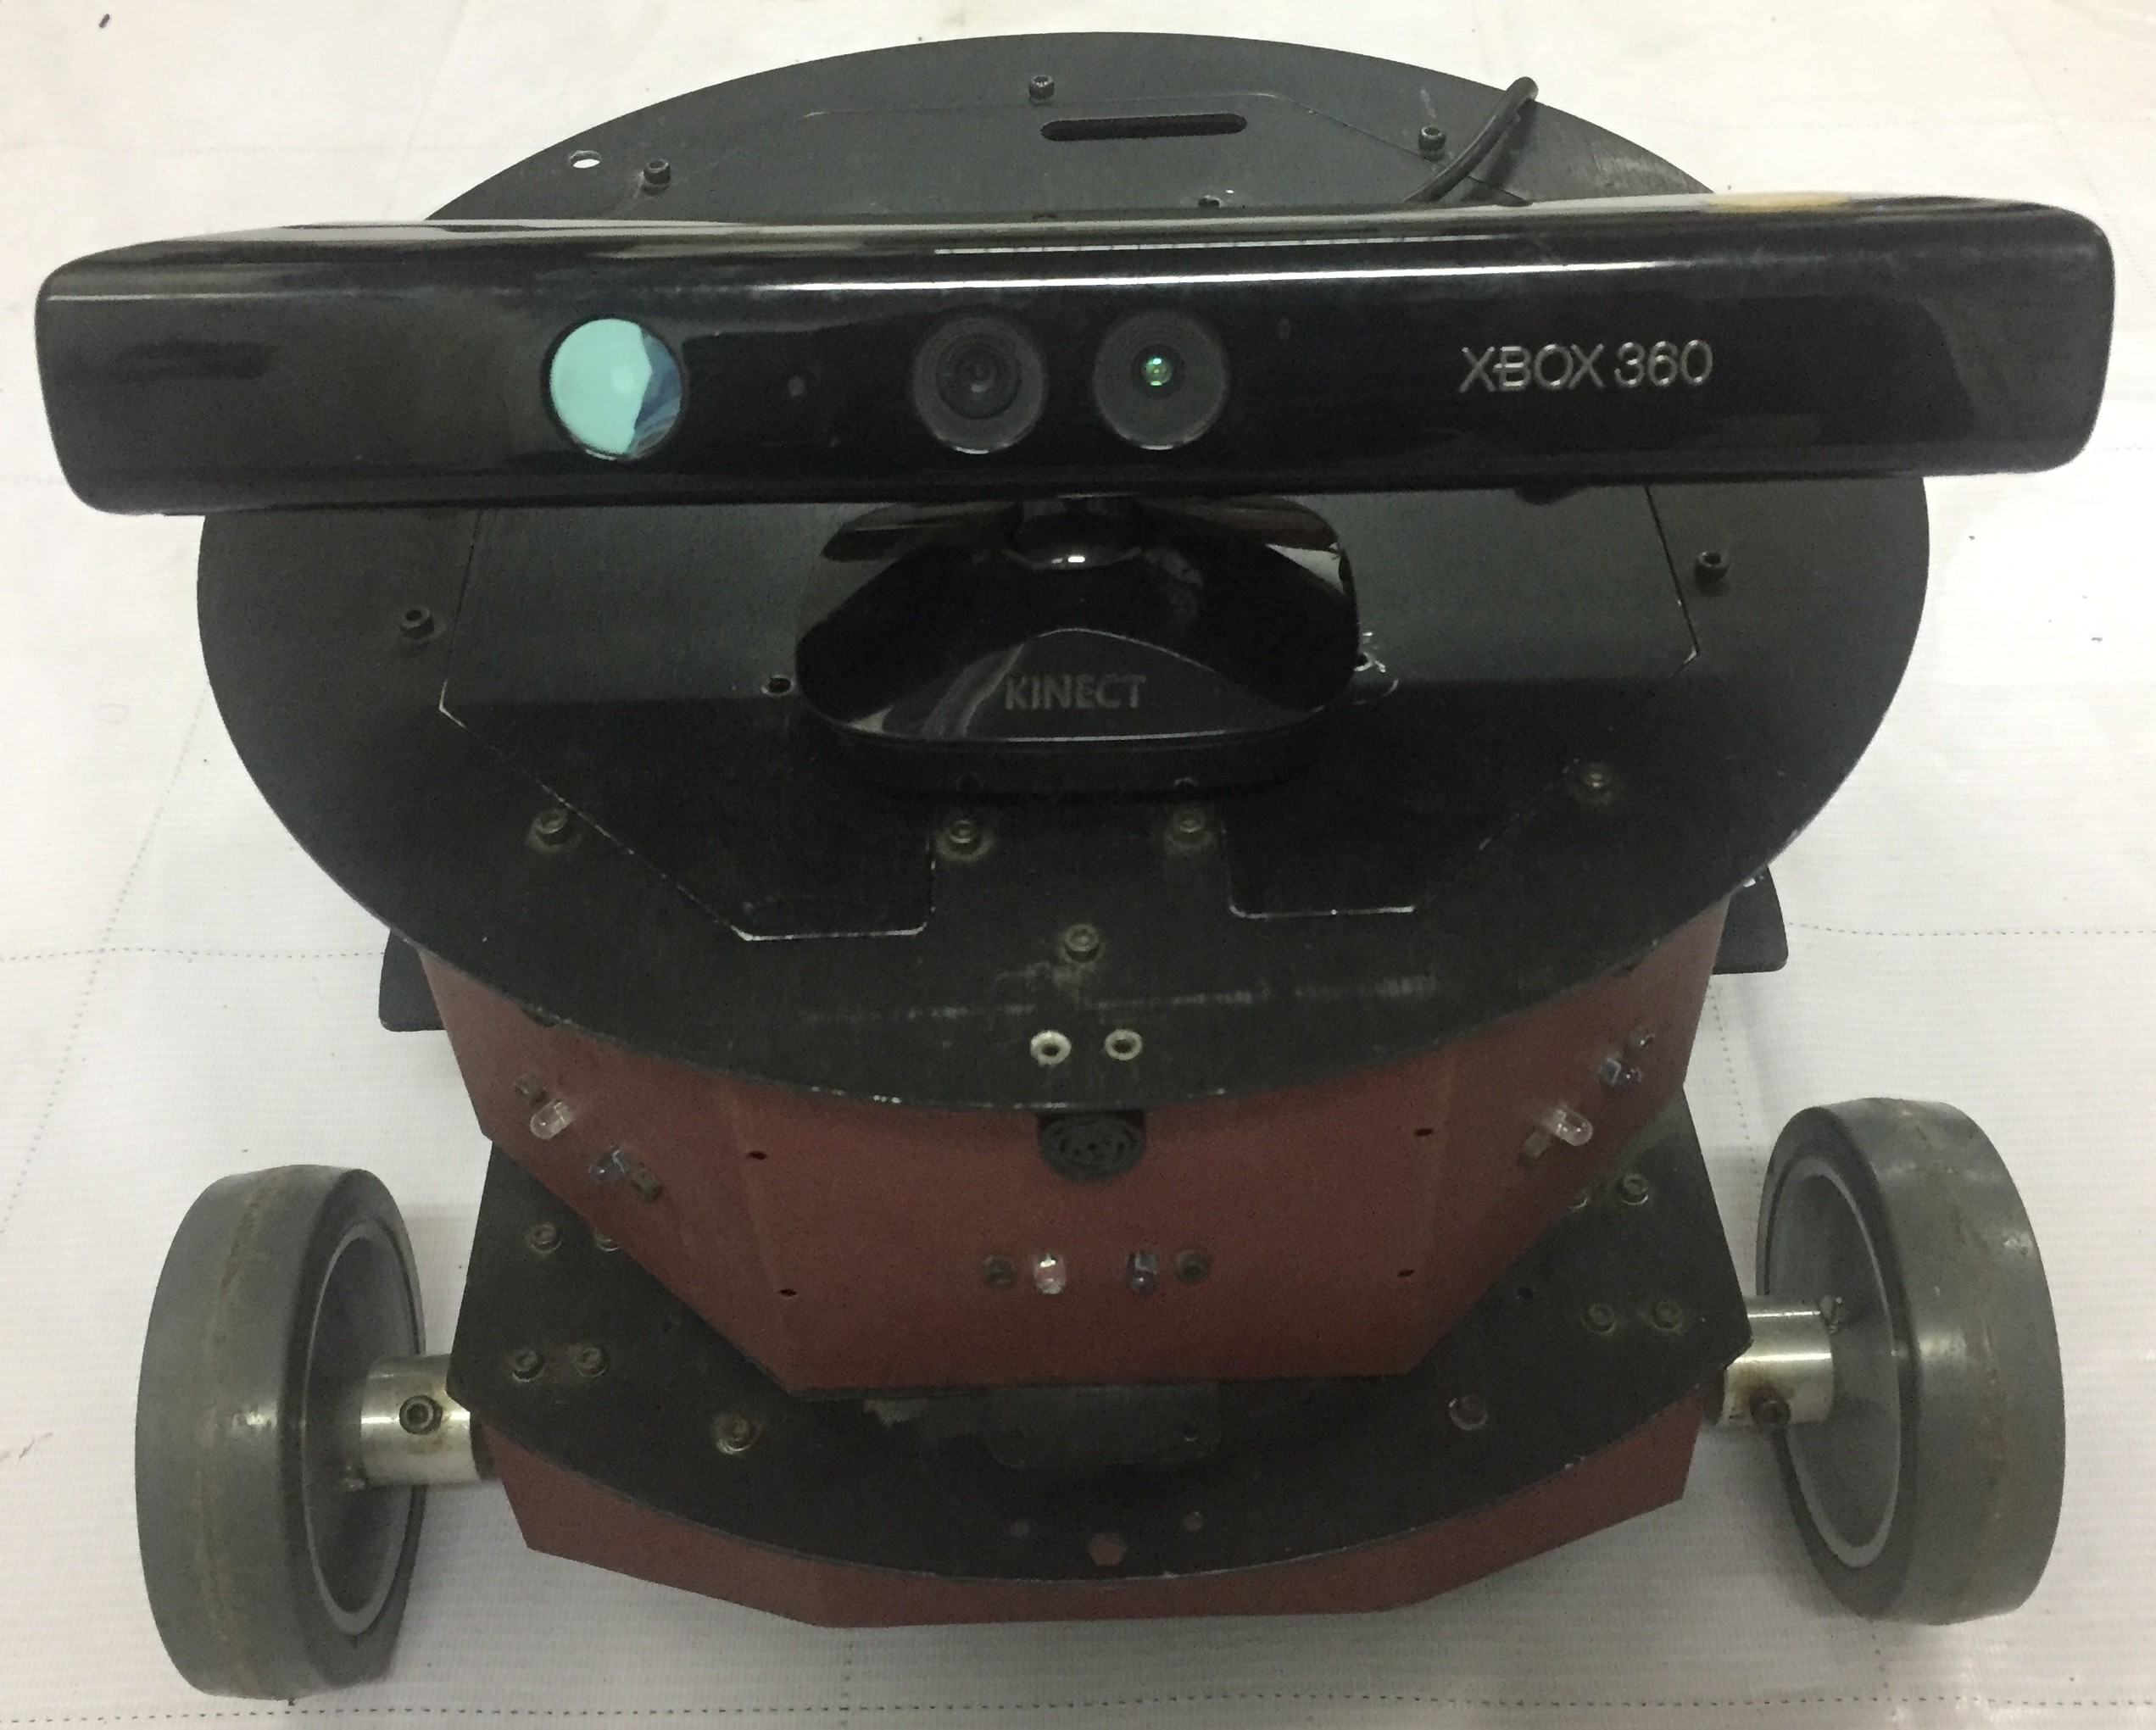
\includegraphics[scale=0.08]{bot}
	\caption{Final setup}
\end{figure}

\pagebreak

\begin{figure}[h]
	\centering
	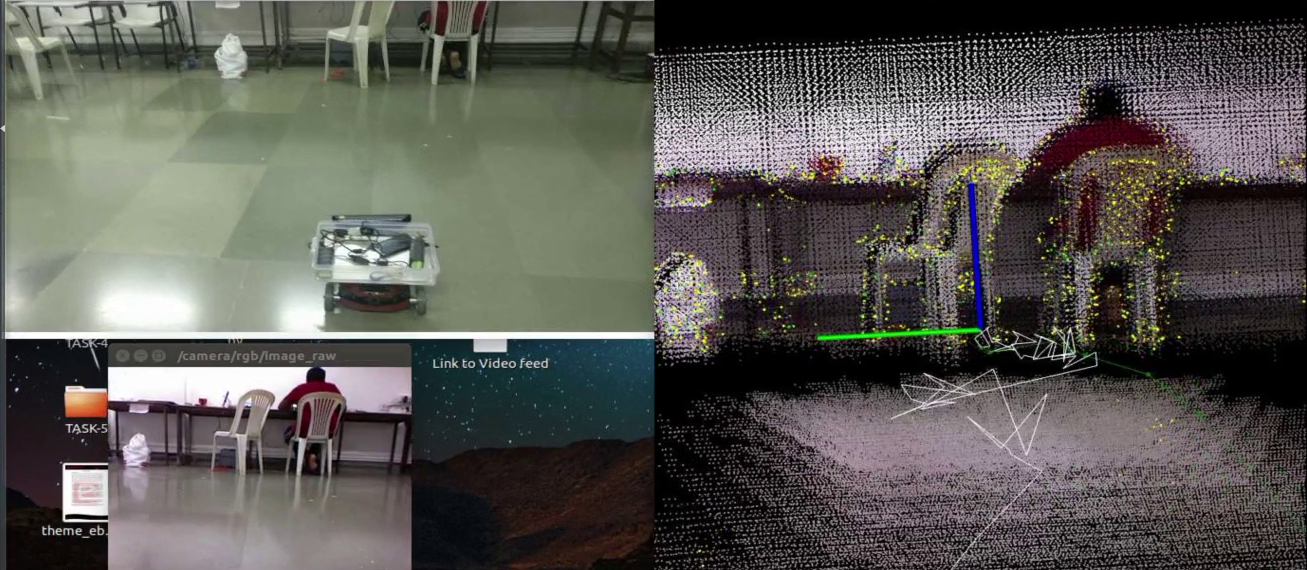
\includegraphics[scale=0.4]{botmap}
	\caption{Result of manual mapping in the real world}
\end{figure}

\href{https://youtu.be/IJxsbCbQITg}{Demonstration video for manual mapping of the real world}

\section{Future Work}
	\begin{itemize}
		\item Autonomous mapping of the real world using a Firebird VI robot or a quadcopter.
		\item Build a system comprising of two drones/robots where one of them maps the environment autonomously, while the other navigates autonomously in the generated map to perform a simple task.
	\end{itemize}

\section{Bug report and Challenges}
\begin{itemize}
	\item Issues:
		\begin{itemize}
			\item The mass of the Realsense R200 camera was set to 1 gram in Gazebo. Setting it to a higher value increases the load on the drone, which causes a constant decrease in altitude.
			\item When the drone goes very close to an obstacle in Gazebo, the camera is able to see through the obstacle and hence pointclouds which would be impossible to generate in the real world are generated in the simulated world.
			\item Due to the numerous front-end and back-end processes running, the processor(i5 5th Gen Dual-Core) was overloaded. This created a huge delay between the generation of pointclouds and the map building process.
			\item The MoveIt package was developed for robotic arms. Hence, when using the package for a drone, the planned trajectories are overly complex.
		\end{itemize}

	\item Failures:
		\begin{itemize}
			\item Due to compatibility issues with the RGB-D camera and the processor, the original idea of mapping with a drone in the real world had to be dropped. Hence, we used a Firebird VI robot for manual mapping.
		\end{itemize}
		
	\item Challenges faced:
		\begin{enumerate}
			\item Problem: ROS comes pre-installed with Gazebo2, but the Realsense plugin works only with Gazebo7 and higher. \\
			Solution: Replaced Gazebo2 with Gazebo7.
			\item Setting the right values for the PID parameters
			\item Problem: The Gazebo plug-in for Realsense camera does not publish camera metadata and calibration parameters(camera info) \\
			Solution: Wrote a python script to publish camera info (obtained from the physical realsense camera) for depth and color cameras in sync with the image data
			\item Problem: The default encoding of the depth image is mono16, which is not supported by the depth\_image\_proc nodelets \\
			Solution: Changed the encoding of the depth image from mono16 to 16UC1 using the toCvShare function of the cv\_bridge library
			\item Problem: Register nodelet of depth\_image\_proc requires a transform from the depth image to the color image \\
			Solution: Created a static\_transform\_publisher node to publish tf data (based on placement of the depth and color cameras in the SDF model of the realsense camera)
			\item Problem: Choosing between the octomap package and rtabmap package of ROS to build a map \\
			Solution: Octomaps require a localization process(e.g. hector\_mapping) running in the background, whereas RTAB-Map runs a SLAM algorithm based on loop closure detection for localization and mapping. Hence we chose to use RTAB-Map to create a map of the environment
			\item Problem: Choosing an efficient algorithm for autonomous mapping \\
			Solution: Two options were available - Wall following, and frontier-based exploration. We chose frontier-based exploration because, the wall following strategy was limited to only rectangular walls and does not perform well with obstacles in the map.
			\item Problem: Choosing a good clustering technique for the frontier-based exploration algorithm \\
			Solution: We chose the k-means clustering algorithm to cluster the frontier cells, because it is one of the most efficient clustering algorithms for big data sets and the clusters generated are of similar sizes
			\item Problem: Choosing an optimal value of K in the k-means clustering algorithm \\
			Solution: The efficiency of the entire algorithm depends on the value of K (number of clusters). A very low value of K would give us large clusters which would be useless given that the drone has a limited field of view. A large value of K would give us very small clusters, which would slow down the mapping process. Hence, we fixed an upper limit on the number of frontier cells each cluster can accommodate, and found the value of K.
		\end{enumerate}
\end{itemize}

\begin{thebibliography}{li}

\bibitem{labbe14online}
Labbe, M. and Michaud, F.,
{\em Online Global Loop Closure Detection for Large-Scale Multi-Session Graph-Based SLAM},
2014

\bibitem{labbe13appearance}
Labbe, M. and Michaud, F.,
{\em Appearance-Based Loop Closure Detection for Online Large-Scale and Long-Term Operation},
2013

\bibitem{}
Cheng Zhu, Rong Ding, Mengxiang Lin, Yuanyuan Wu,
{\em A 3D frontier-based exploration tool for MAVs},
2015

\bibitem{}
\href{http://wiki.ros.org}{ROS Wiki}

\bibitem{}
\href{http://gazebosim.org/}{Gazebo simulator}

\bibitem{}
\href{https://introlab.github.io/rtabmap/}{RTAB-Map}

\bibitem{}
\href{http://moveit.ros.org/}{MoveIt!}

\bibitem{}
\href{https://www.wilselby.com/research/ros-integration/3d-mapping-navigation/}{MoveIt for quadrotors}

\bibitem{}
\href{http://www.sealevel.com/store/media/catalog/product/cache/1/image/9df78eab33525d08d6e5fb8d27136e95/d/b/db9m-rs232-pinout.jpg}{RS232 Connector}

\end{thebibliography}


\end{document}

